\addtocontents{toc}{\protect\setcounter{tocdepth}{2}}
\section{History}
Here an attempt will be made to very briefly highlight some of the ideas, features and syntax of a number of languages. The classification is quite arbitrary as most languages support multiple paradigms.
\section{Assembly languages}
RISC >< CISC
\subsection{M32}
\subsection{Z80}
\subsection{(M)MIX}
\subsection{x86}
\subsection{ARM}

\section{Procedural languages}
\subsection{FORTRAN 77}
\paragraph{History.}
FORTRAN (FORmula TRANslation) was the first high-level programming language to become widely used. At conception, in 1957, there were serious concerns as to whether a high-level language could ever seriously compete with assembly languages. Thus design was oriented heavily towards efficiency.

The language went through many revisions. The biggest change was between FORTRAN 77 and Fortran 90. Fortran 95 is the most widely implemented of the more recent specifications and later versions are largely similar.

\paragraph{Syntactic features.}
The basic structure of a program can be seen in this hello world example.
\begin{lstlisting}[language={[77]fortran}, style=program]
      program helloworld
        print *, "Hello world!"
        stop
        end
\end{lstlisting}
The \texttt{stop} statement is optional since the program will stop when it reaches the end, but is recommended to emphasize that execution flow stops there. You cannot have a variable with the same name as the program.

FORTRAN is completely case insensitive and was traditionally written in all caps. Current practice is to mix upper and lower case.

Blanks are ignored completely, in fact they may all be removed. Spaces may be inserted freely.

FORTRAN 77 uses fixed-format source code:
\begin{itemize}
\item Comments must begin with a \texttt{C} or a \texttt{*} in column 1. Some compilers allow in-line comment with an \texttt{!}. The exclamation mark may appear anywhere on a line, except in positions 2-6.
\item Statement labels must occur in columns 1-5
\item Continuation lines must have a non-blank character in column 6. Any non-blank character can be used as a continuation character. Traditionally a plus, an ampersand or a digit is used. Example:
\begin{lstlisting}[language={[77]fortran}, style=snippet]
c The next statement goes over two physical lines
      area = 3.14159265358979
     +       * r * r
\end{lstlisting}
\item Statements must start in column 7.
\item The line-length may be limited to 72 characters (derived from the 80-byte width of a punch-card, with last 8 characters reserved for (optional) sequence numbers)
\end{itemize}



\subparagraph{Variables, types and declarations}
Variables are 1 to 6 characters long, begin with a letter and may contain letters and digits.

Reserved words are: \texttt{assign, backspace, block data, call, close, common, continue, data, dimension, do, else, else if, end, endfile, endif, entry, equivalence, external, format, function, goto, if, implicit, inquire, intrinsic, open, parameter, pause, print, program, read, return, rewind, rewrite, save, stop, subroutine, then, write}.

Variables do not have to be explicitly declared. Explicit declarations take the form
\begin{lstlisting}[language={[77]fortran}, style=snippet]
      integer A, B, C
      real radius, eulerE
      double precision q, r
      complex z
      logical t
      character ch
\end{lstlisting}
If there is no explicit declaration, a \textit{naming convention} is used. By default variable names beginning with \texttt{I-N} are integer variables; all others are real. This default behaviour can be modified with an \texttt{IMPLICIT} statement:
\begin{lstlisting}[language={[77]fortran}, style=snippet]
      IMPLICIT INTEGER (A-Z)
\end{lstlisting}
This causes the type integer to be assumed for all variables.

Constants are defined in the following way
\begin{lstlisting}[language={[77]fortran}, style=snippet]
      PARAMETER (KMAX = 100, MIDPT = 50)
\end{lstlisting}
the \texttt{parameter} statement(s) must come before the first executable statement.

\subparagraph{Arrays.} One-dimensional arrays are declared as follows.
\begin{lstlisting}[language={[77]fortran}, style=snippet]
      real a(20)
      real b(0:19), weird(-162:237)
      double precision x(100)
\end{lstlisting}
By default arrays are indexed from $1$ to their length, inclusive. Arbitrary index ranges can also be defined, see arrays \texttt{b} and \texttt{wierd} above.

Elements or arrays can be accessed using brackets: \texttt{a(3) = 2.0}. The Fortran compiler does not check whether array elements are out of bounds or undefined!

Multi-dimensional arrays can be declared in a similar way by putting a comma between indexes:
\begin{lstlisting}[language={[77]fortran}, style=snippet]
      real A(3,5,2:7)
      A(1,4,2) = 5
\end{lstlisting}

Two-dimensional arrays are stored in memory as contiguous sequences of elements, column by column.

An alternative (old-fashioned) style is to use the \texttt{dimension} statement:
\begin{lstlisting}[language={[77]fortran}, style=snippet]
      real A, x
      dimension x(50)
      dimension A(10,20)
C This is equivalent to:
      real A(10,20), x(50)
\end{lstlisting}

\subparagraph{The \texttt{DATA} statement} is a compact way to input data that is known at compile time. The syntax is as follows
\begin{lstlisting}[language={[77]fortran}, style=snippet]
      data m/10/, n/20/, x/2.5/, y/2.5/
C Or alternatively
      data m,n/10,20/, x,y/2*2.5/
\end{lstlisting}
Both statements result in \texttt{m = 10, n = 20, x = 2.5, y = 2.5}.

The data statement is performed only once, right before the execution of the program starts. For this reason, the data statement is mainly used in the main program and not in subroutines. It can also be used to initialize arrays (vectors, matrices).
\begin{lstlisting}[language={[77]fortran}, style=snippet]
      real A(10,20)
      data A/ 200 * 0.0/
C Individual elements may also be initialised
      data A(1,1)/ 12.5/, A(2,1)/ -33.3/, A(2,2)/ 1.0/
\end{lstlisting}

The data statement cannot be used for variables contained in a common block. There is a special syntax for this purpose, called \texttt{block data}.
\begin{lstlisting}[language={[77]fortran}, style=snippet]
      block data
        integer nmax
        parameter (nmax=20)
        real v(nmax), alpha, beta
        common /vector/v,alpha,beta
        data v/20*100.0/, alpha/3.14/, beta/2.71/
      end
\end{lstlisting}

The block data may not be nested inside the main program or a subroutine.

\paragraph{Expressions and assignment}
FORTRAN supports the following literals:
\begin{itemize}
\item Integer literals
\begin{lstlisting}[language={[77]fortran}, style=snippet]
      1
      0
      -100
      32767
      +15
\end{lstlisting}
\item Real literals
\begin{lstlisting}[language={[77]fortran}, style=snippet]
      1.0
      -0.25
      2.6E6
      3.333E-1
\end{lstlisting}
The $E$ means multiply by $10$ to the power of whatever comes after it.
\item Double precision literals
\begin{lstlisting}[language={[77]fortran}, style=snippet]
      2.0D-1
      1D99
\end{lstlisting}
Like reals, but $D$ instead of $E$.
\item Complex literals
\begin{lstlisting}[language={[77]fortran}, style=snippet]
      (2, -3)
      (1., 9.9E-1)
\end{lstlisting}
\item Logical literals
\begin{lstlisting}[language={[77]fortran}, style=snippet]
      .TRUE.
      .FALSE.
\end{lstlisting}
\item Character literals. Most often used in arrays (as strings). Some versions of FORTRAN require single quotes.  An enclosed single-quote can be represented by doubling.
\begin{lstlisting}[language={[77]fortran}, style=snippet]
      'ABC'
      'Anything goes!'
      'It''s a nice day'
\end{lstlisting}
\end{itemize}

Operator precedence in FORTRAN 77 (from highest to lowest):
\begin{enumerate}
\item[\texttt{**}] Exponentiation
\item[\texttt{-}] Unary minus
\item[\texttt{*, /}] Multiplication, division
\item[\texttt{+,-}] Addition, subtraction
\item[] Relational operators: \texttt{.LT., .LE., .GT., .GE., .EQ., .NE.} (respectively $<, <=, >, >=, =, \backslash=$).
\item[\texttt{.NOT.}] Logical not
\item[\texttt{.AND.}] Logical and
\item[\texttt{.OR.}] Logical or
\end{enumerate}
For different evaluation order, use parentheses.

Caution must be taken when using the \undline{division operator}. If both operands are integer, integer division is performed, otherwise real arithmetic division is performed.

Assignment is done with the equals sign
\begin{lstlisting}[language={[77]fortran}, style=snippet]
      area = pi * r**2
\end{lstlisting}

For type conversion, the following functions are available: \texttt{int(), real(), dble(), ichar(), char()}. The function \texttt{ichar} converts a character into an integer; \texttt{char} does the opposite.

Constructs that are not statically checked are ordinarily left unchecked.

\paragraph{Flow control.}
The \texttt{if} statement comes in several forms:
\begin{lstlisting}[language={[77]fortran}, style=snippet]
      if (x .LT. 0) x = -x
\end{lstlisting}
or
\begin{lstlisting}[language={[77]fortran}, style=snippet]
      if (x .LT. 0) then
        x = -x
      endif
\end{lstlisting}
or
\begin{lstlisting}[language={[77]fortran}, style=snippet]
      if (x .LT. 0) then
        x = -x
      elseif (x .GT. 5) then
        x = 5
      else
        x = x+1
      endif
\end{lstlisting}
\texttt{if} statements can also be nested.

FORTRAN 77 only has the \texttt{do}-loop. An example:
\begin{lstlisting}[language={[77]fortran}, style=snippet]
      integer i, n, sum
 
      sum = 0
      do 10 i = 1, n
         sum = sum + i
         write(*,*) 'i =', i
         write(*,*) 'sum =', sum
  10  continue
\end{lstlisting}
Here the number $10$ is a label. Column positions 1-5 are reserved for statement labels. Typically, most programmers use consecutive multiples of 10.

The \texttt{continue} statement is a placeholder that does nothing.

The statement identified by the label after the \texttt{DO} command is called the \udef{terminal statement}.

The variable is typically incremented by one each loop until the second value is reached (inclusive). A step may also be specified (negative means counting down).
\begin{lstlisting}[language={[77]fortran}, style=snippet]
      integer i
 
      do 20 i = 10, 1, -2
         write(*,*) 'i =', i
  20  continue
\end{lstlisting}

Many compilers also allow the \texttt{DO} statement to be closed by \texttt{ENDDO}. This is not ANSI FORTRAN 77, however. The expressions in the beginning of the \texttt{DO}-loop arwe evaluated only once. So the following loop does not run forever:
\begin{lstlisting}[language={[77]fortran}, style=snippet]
      integer i,j
 
      read (*,*) j
      do 20 i = 1, j
         j = j + 1
  20  continue
      write (*,*) j
\end{lstlisting}

Other types of loops have to be simulated using \texttt{GOTO} statements.
\begin{lstlisting}[language={[77]fortran}, style=snippet]
     integer n

     n = 1
  10 if (n .LE. 100) then
        write (*,*) n
        n = 2*n
        goto 10
     endif
\end{lstlisting}

\paragraph{Subprograms.}
Fortran has two different types of subprograms, called functions and subroutines. 

Functions take a set of input arguments (parameters) and return a value of some type.
Some built-in functions include:
\begin{lstlisting}
abs     absolute value
min     minimum value
max     maximum value
sqrt    square root
sin     sine
cos     cosine
tan     tangent
atan    arctangent
exp     exponential (natural)
log     logarithm (natural)
\end{lstlisting}

An example of a user-defined function:
\begin{lstlisting}[language={[77]fortran}, style=snippet]
      real function r(m,t)
        integer m
        real t
        r = 0.1*t * (m**2 + 14*m + 46)
        if (r .LT. 0) r = 0.0
        return
      end
\end{lstlisting}
We see
\begin{itemize}
\item Functions have a type. If none is declared, the same implicit typing system as for variables is used.
\item Functions are terminated by the \texttt{return} statement.
\item The return value should be stored in a variable with the same name as the function. 
\item Strictly speaking Fortran 77 does not permit recursion. However, it is not uncommon for a compiler to allow recursion. 
\end{itemize}

A subroutine does not return a value. The syntax is as follows:
\begin{lstlisting}[language={[77]fortran}, style=snippet]
      subroutine iswap (a, b)
        integer a, b
        integer tmp
        tmp = a
        a = b
        b = tmp
        return
      end
\end{lstlisting}
The subroutine works because parameters in FORTRAN 77 subprograms are \undline{passed by reference.}

We can pass arrays of arbitrary size to subprograms if we define the arrays in the subprogram with dummy indices (usually an asterisk).

\paragraph{Common blocks and scope.}
FORTRAN 77 has no global variables. Common blocks can be used instead. In general the syntax is as follows
\begin{lstlisting}[language={[77]fortran}, style=snippet]
      program main
        real alpha, beta
        common /coeff/ alpha, beta
        [ statements ]
        stop
      end
C
      subroutine sub1 ( [ some arguments ] )
        [ declarations of arguments ]
        real alpha, beta
        common /coeff/ alpha, beta
        [ statements ]
        return
      end
C
      subroutine sub2 ( [ some arguments ] )
        [ declarations of arguments ]
        real alpha, beta
        common /coeff/ alpha, beta
        [ statements ]
        return
      end
\end{lstlisting}
The syntax of a common statement is: \texttt{COMMON / name / list-of-variables}. A variable cannot belong to more than one common block. The variables in a common block do not need to have the same names each place they occur (although it is a good idea to do so), but they must be listed in the same order and have the same type and size.

Putting arrays in common blocks is a bad idea.
\paragraph{I/O.} In FORTRAN each file is associated with a unit number, an integer between 1 and 99. Some unit numbers are reserved: 5 is standard input, 6 is standard output. 

Before you can use a file you have to open it. The command is 
\begin{lstlisting}[language={[77]fortran}, style=snippet]
      open (list-of-specifiers)
\end{lstlisting}
Where the most common specifiers are
\begin{lstlisting}
[UNIT=]  u
IOSTAT=  ios
ERR=     err
FILE=    fname
STATUS=  sta
ACCESS=  acc
FORM=    frm
RECL=    rl
\end{lstlisting}
\begin{itemize}
\item[\texttt{u}]  is a number between 1 and 99 inclusive that denotes the file.
\item[\texttt{ios}] is the I/O status identifier and should be an integer variable. Upon return, \texttt{ios} is set to zero if the statement was successful and set to a non-zero value otherwise. 
\item[\texttt{err}] is a label which the program will jump to if there is an error. 
\item[\texttt{fname}] is a character string denoting the file name. 
\item[\texttt{sta}] is a character string that has to be either \texttt{NEW}, \texttt{OLD} or \texttt{SCRATCH}. It shows the prior status of the file. A scratch file is a file that is created when opened and deleted when closed (or the program ends). 
\item[\texttt{acc}] must be either \texttt{SEQUENTIAL} or \texttt{DIRECT}. The default is \texttt{SEQUENTIAL}.
\item[\texttt{frm}] must be either \texttt{FORMATTED} or \texttt{UNFORMATTED}. The default is \texttt{UNFORMATTED}. 
\item[\texttt{rl}] specifies the length of each record in a direct-access file. 
\end{itemize}
After a file has been opened, you can access it by read and write statements. When you are done with the file, it should be closed by the statement 
\begin{lstlisting}[language={[77]fortran}, style=snippet]
      close ([UNIT=]u[,IOSTAT=ios,ERR=err,STATUS=sta])
\end{lstlisting}
In this case \texttt{sta} is a character string which can be \texttt{KEEP} (the default) or \texttt{DELETE}. 

Reading and writing is done as follows:
\begin{lstlisting}[language={[77]fortran}, style=snippet]
read ([UNIT=]u, [FMT=]fmt, IOSTAT=ios, ERR=err, END=s) [ list-of-variables ]
write([UNIT=]u, [FMT=]fmt, IOSTAT=ios, ERR=err, END=s) [ list-of-variables ]
\end{lstlisting}
The \texttt{END=s} specifier defines which statement label the program jumps to if it reaches end-of-file. The format number \texttt{fmt} refers to a label for a format statement (described below).

The first two arguments can be replaced with asterisks. This is sometimes called \udef{list directed} read / write. This format assumes the file has a line per record and the fields are separated by blanks or commas.

If we are reading or writing to the stantard input, the followinf syntax may be used (the asterisk refers to the format):
\begin{lstlisting}[language={[77]fortran}, style=snippet]
      read  *, [ list-of-variables ]
      print *, [ list-of-variables ]
\end{lstlisting}

\paragraph{The \texttt{FORMAT} statement} TODO

\paragraph{Language design notes}

Changes compared to FORTRAN 66:
\begin{itemize}
\item Additions:
\begin{itemize}
\item Block \texttt{IF} and \texttt{END IF} statements, with optional \texttt{ELSE} and \texttt{ELSE IF}.
\item \texttt{DO}-loop extensions including
\begin{itemize}
\item parameter expressions
\item negative increments
\item zero trip counts
\item Better file I/O.
\item The \texttt{IMPLICIT} statement.
\item The \texttt{PARAMETER} statement.
\item The \texttt{CHARACTER} datatype.
\item Lexical comparison of strings with \texttt{LGE, LGT, LLE, LLT}.
\end{itemize}
\end{itemize}
\item Deprecated:
\begin{itemize}
\item Hollerith constants and Hollerith data.
\item Transfer of control out of and back into the range of a DO loop (also known as "Extended Range")
\end{itemize}
\end{itemize}
\subsection{Fortran 95}
Changes compared to Fortran 90:
\begin{itemize}
\item Additions:
\begin{itemize}
\item 
\end{itemize}
\item Deprecated:
\begin{itemize}
\item
\end{itemize}
\item Changes:
\begin{itemize}
\item 
\end{itemize}
\end{itemize}
Changes in FORTRAN 2003:
\begin{itemize}
\item Additions:
\begin{itemize}
\item 
\end{itemize}
\item Deprecated:
\begin{itemize}
\item
\end{itemize}
\item Changes:
\begin{itemize}
\item 
\end{itemize}
\end{itemize}
Changes in FORTRAN 2008:
\begin{itemize}
\item Additions:
\begin{itemize}
\item 
\end{itemize}
\item Deprecated:
\begin{itemize}
\item
\end{itemize}
\item Changes:
\begin{itemize}
\item 
\end{itemize}
\end{itemize}
Changes in FORTRAN 2018:
\begin{itemize}
\item Additions:
\begin{itemize}
\item 
\end{itemize}
\item Deprecated:
\begin{itemize}
\item
\end{itemize}
\item Changes:
\begin{itemize}
\item 
\end{itemize}
\end{itemize}
\subsection{C}
\subsection{Pascal}
Of course, in stupid languages like Pascal, where labels cannot be
descriptive, GOTOs can be bad. But that's not the fault of the goto,
that's the braindamage of the language designer.


\subsection{SNOBOL}
\subsubsection{History}
Development of SNOBOL (StriNg Oriented and symBOlic Language) began in 1962 at AT\&T Bell Labs by Ralph Griswold, Ivan Polonsky and David Farber. The goal was to develop a string processing language for formula manipulation and graph analysis. The most successful version was SNOBOL4, developed in the 1970s.

SPITBOL (Speedy Implementation of SNOBOL) is a compiled implementation of the SNOBOL4.
\subsubsection{Concepts}
\begin{itemize}
\item Pattern matching language based upon BNF Grammars.
\item Patterns are a first-class data type.
\end{itemize}
\subsection{Go}

\section{UML}
\subsection{What is it?}
The Unified Modeling Language (UML) is a family of graphical notations that help describing and designing software systems, particularly software systems built using the object-oriented paradigm. The UML is a relatively open standard, controlled by the Object Management Group (OMG), an open consortium of companies. The UML was born out of the unification of many graphical modeling languages around in the late 1980s and early 1990s.

\subsubsection{Ways of using it}
One can identify three modes in which UML is often used:
\begin{enumerate}
\item \textbf{UML as a sketch.} In this usage UML is used to communicate some aspect of a system. Such a sketch is by no means complete, but just meant to illustrate an idea. Selectivity is key.
\item \textbf{UML as a blueprint.} In this usage the UML diagram is meant to be a complete and detailed guide to the code. A blueprint may be of the whole system or of a particular area. Such diagrams can be used by specialised \udef{CASE (computer aided software engineering) tools}.
\item \textbf{UML as a programming language} is when the blueprint is complete and accurate enough that it can mechanically be converted into executable code. The standard approach is called \udef{Model-Driven Architecture (MDA)}. 
\end{enumerate}

The UML can also be used for conceptual modeling or software modeling.
\begin{enumerate}
\item In the \textbf{software perspective}, the UML elements map (fairly) directly to elements in the software system. Within the software perspective, a distinction can also be made between diagrams focusing on \textit{interface} or \textit{implementation}.
\item In the \textbf{conceptual perspective}, the diagram deals in concepts, not necessarily actual components in the system.
\end{enumerate}

The UML standard can also be seen as having either \textit{prescriptive} or \textit{descriptive} rules. TODO Fowler p.13

\subsubsection{Notation and meta-model}
The UML defines
\begin{itemize}
\item a \textbf{notation} (i.e. graphical syntax) and
\item a \textbf{meta-model} which defines the concepts of the language.
\end{itemize}
When referring to the UML, sometimes the notation and sometimes the meta-model is meant.

\subsubsection{UML diagrams}

\subsection{Class diagrams}
\begin{wrapfigure}{r}{0.3\textwidth}
\vspace{-10pt}
\begin{tikzpicture}
\umlclass{Order}{
  dateReceived : Date[0..1] \\ isPrepaid: Boolean[1] \\ number: String[1] \\ price: Money
}{dispatch \\ close}
\end{tikzpicture}
\vspace{-20pt}
\end{wrapfigure}

A class diagram describes the various types of objects in the system and the static relationships that exist among them. Each class has a name and several \udef{features}, i.e. the properties and operations of a class. 

\subsubsection{Properties}
\udef{Properties} represent the structural features of a class. Properties appear in two very distinct notations: \textit{attributes} and \textit{associations}.

\paragraph{Attributes} define the property within the class box itself. They are put in the section under the title. The full form of an attribute is:
\begin{syntax}
\opt{\textit{visibility}} \opt{/} \textit{name} \opt{: \textit{type}} \opt{[\textit{multiplicity}]} \opt{= \textit{default}} \opt{\textit{property-string}}
\end{syntax}
Only \texttt{\textit{name}} is necessary.
\begin{itemize}
\item \texttt{\textit{visibility}} can be
\begin{itemize}
\item \texttt{+} for public
\item \texttt{-} for private
\item \texttt{$\sim$} for package
\item \texttt{\#} for protected
\end{itemize}
\item \texttt{/} means the property is a derived property, i.e. calculated from other properties.
\item \texttt{\textit{name}} is the name of the attribute.
\item \texttt{\textit{type}} indicates what kind of object may be placed in the attribute.
\item \texttt{\textit{multiplicity}} shows how many objects may fill the property. Multiplicities may be specified as
\begin{itemize}
\item \texttt{\textit{number}}: the property contains \texttt{\textit{number}} objects.
\item \texttt{\textit{lowerBound}..\textit{upperBound}}: the property contains more than \texttt{\textit{lowerBound}}, but no more than \texttt{\textit{upperBound}}, objects.
\item \texttt{*}: the property contains an arbitrary number (zero or more) of objects.
\item \texttt{\textit{lowerBound}..*}: the property contains more than \texttt{\textit{lowerBound}} objects.
\end{itemize}
\item \texttt{\textit{number}} is the value for a newly created object if the attribute is not specified during creation.
\item \texttt{\textit{property-string}} is of the form
\begin{syntax}
\{ \textit{property-modifier} \mult{, \textit{property-modifier}} \}
\end{syntax}
where \texttt{\textit{property-modifier}} can be one of
\begin{itemize}
\item \texttt{id}: the property is part of the identifier for the class which owns the property.
\item \texttt{readOnly}: clients may not modify the property.
\item \texttt{ordered} or \texttt{unordered}: the objects associated with this multi-valued property are (un)ordered.
\item \texttt{unique} or \texttt{nonunique}: the objects associated with this multi-valued property may or may not have duplicate values.
\item \texttt{sequence} (or \texttt{seq}): \texttt{ordered} and \texttt{nonunique}.
\item \texttt{bag}: \texttt{unordered} and \texttt{nonunique}.
\item \texttt{union}: the property is a derived union of its subsets TODO?.
\item \texttt{redefines \textit{property-name}}: the property redefines an inherited property named \texttt{\textit{property-name}}.
\item \texttt{subsets \textit{property-name}}: the property is a subset of the property named \texttt{\textit{property-name}}.
\item \texttt{\textit{property-constraint}}: A constraint that applies to the property.
\end{itemize}
\end{itemize}

\paragraph{Associations} are another way to notate properties. An \udef{association} is a solid line between two classes, directed from the source class to the target class. All extra information about the property is written at the target end of the association.

\begin{figure}
\centering
\begin{subfigure}{.5\textwidth}
  \centering
  \begin{tikzpicture}
\umlclass{Order}{
  + dateReceived : Date[0..1] \\ + isPrepaid: Boolean[1] \\ + lineItems: OrderLine[*] {ordered}
}{}
\end{tikzpicture}
  \caption{Showing properties as attributes}
  \label{fig:attributesAssociations:sub1}
\end{subfigure}%
\begin{subfigure}{.5\textwidth}
  \centering
  \begin{tikzpicture}
\umlsimpleclass{Date}
\umlsimpleclass[x=4]{Order}
\umlsimpleclass[x=8]{Boolean}
\umlsimpleclass[y=-2, x=4]{OrderLine}
\umluniassoc[attr2=+dateReceived|0..1, mult1=*]{Order}{Date}
\umluniassoc[mult2=1, arg2=+isPrepaid]{Order}{Boolean}
\umluniassoc[mult1=1, mult2=*, arg2={lineItems ordered TODO}]{Order}{OrderLine}
\end{tikzpicture}
  \caption{Showing properties as associations}
  \label{fig:attributesAssociations:sub2}
\end{subfigure}
\caption{The same properties represented in two different notations}
\label{fig:attributesAssociations}
\end{figure}

In general it is useful to use attributes for small things and value types (TODO ref), such as dates and booleans, and associations for more significant classes.

\subsubsection{{Operations}}

\subsection{Sequence diagrams}


\subsection{Executable UML and model-driven architecture}

\section{Object-oriented languages}
\subsection{Ada}
\subsection{C++}
\subsection{Smalltalk}
\subsection{Java}
\subsection{Scala}
\paragraph{History}
Released in 2004 by Martin Odersky. Provides support for functional programming. Designed to be compiled to Java bytecode, so that Scala applications can be executed on a Java Virtual Machine (JVM).

\paragraph{Basic setup}
Scala has a tool called the REPL (Read-Eval-Print Loop) that is analogous to
  commandline interpreters in many other languages. You may type any Scala
  expression, and the result will be evaluated and printed.

Results are saved as values and may be used in future expressions.

REPL sessions can be saved and loaded using \texttt{:save [path]} and \texttt{:load [path]}.

Recent history can be shown with \texttt{:h?}.

Full programs have the following form. The entry point is defined using an object with a single method, \texttt{main}.
\begin{lstlisting}[language=scala, style=program]
object Application {
  def main(args: Array[String]): Unit = {
    // stuff goes here.
  }
}
\end{lstlisting}

\subparagraph{I/O.} Printing can be done with \texttt{println("Hello world!")}, which forces a newline on next print, or with \texttt{print("Hello world!")}, which does not.

To read a file line by line
\begin{lstlisting}[language=scala, style=snippet]
import scala.io.Source
for(line <- Source.fromFile("myfile.txt").getLines())
  println(line)
\end{lstlisting}

To write a file using Java's \texttt{PrintWriter}
\begin{lstlisting}[language=scala, style=snippet]
val writer = new PrintWriter("myfile.txt")
writer.write("Writing line for line" + util.Properties.lineSeparator)
writer.write("Another line here" + util.Properties.lineSeparator)
writer.close()
\end{lstlisting}

\subparagraph{Importing.}
\begin{lstlisting}[language=scala, style=snippet]
// --- Importing things
import scala.collection.immutable.List
// --- Import all "sub packages"
import scala.collection.immutable._
// --- Import multiple classes in one statement
import scala.collection.immutable.{List, Map}
// --- Rename an import using '=>'
import scala.collection.immutable.{List => ImmutableList}
// --- Import all classes, except some. The following excludes Map and Set:
import scala.collection.immutable.{Map => _, Set => _, _}
// --- Java classes can also be imported. Scala syntax can be used
import java.swing.{JFrame, JWindow}
\end{lstlisting}


\paragraph{Syntactic elements}

Comments:
\begin{lstlisting}[language=scala, style=snippet]
// Single line comment
/*
Multiline
comment
*/
\end{lstlisting}

Scala is strongly typed. Types can be checked without evaluating the expression. (This can be done in the REPL with \texttt{:type}).

\subparagraph{Blocks}
Expressions can be combined by surrounding them with braces \texttt{\{\}}.
\begin{lstlisting}[language=scala, style=snippet]
println(7) // Prints 7

println {
  val i = 5
  i + 2
} // Prints 7
\end{lstlisting}

\paragraph{Values, variables and data types}
Values are like immutable variables, variables are mutable. Declaration is done with the \texttt{val} and \texttt{var} keywords, respectively.
\begin{lstlisting}[language=scala, style=snippet]
val x = 10 // x is now 10
x = 20     // error: reassignment to val
var y = 10
y = 20     // y is now 20
\end{lstlisting}
Even though Scala is a statically typed language, explicit type declaration is often not needed, due to \textit{type inference}. Explicit type declarations can be done as follows:
\begin{lstlisting}[language=scala, style=snippet]
val z: Int = 10
val a: Double = 1.0
val b: Double = 10
\end{lstlisting}

Scala is considered a pure object-oriented language because every value is an object. Hence there are no primitives in Scala (unlike Java which has ,e.g., \texttt{int}s).

There are eight basic types in Scala: \texttt{Byte, Short, Int, Long, Float, Double, Char, Boolean}.

\begin{figure}[h]
\label{scalaTypeHierarchy}
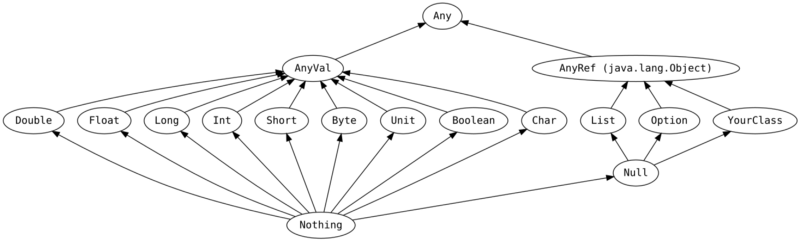
\includegraphics[width=\textwidth]{scalaTypeHierarchy}
\centering
\end{figure}

Every basic Scala type inherits from \texttt{AnyVal}. On the other side, \texttt{AnyRef} is an alias for \texttt{java.lang.Object}. Lastly, both \texttt{AnyVal} and \texttt{AnyRef} inherits from \texttt{Any}.

\subparagraph{Numeric types}:
\begin{lstlisting}[language=scala, style=snippet]
1 + 1   // 2
2 - 1   // 1
5 * 3   // 15
6 / 2   // 3
6 / 4   // 1
6.0 / 4 // 1.5
6 / 4.0 // 1.5
\end{lstlisting}

\subparagraph{Booleans.} Scala supports the Boolean values \texttt{true} an \texttt{false}, as well as the common Boolean operations.
\begin{lstlisting}[language=scala, style=snippet]
!true         // false
!false        // true
true == false // false
10 > 5        // true
\end{lstlisting}

\subparagraph{Strings}
Strings are surrounded by double quotes. Single quotes only used for chars. Triple double-quotes let strings span multiple rows and contain quotes.
\begin{lstlisting}[language=scala, style=snippet]
"Scala strings are surrounded by double quotes"
'a' // A Scala Char
val html = """<form id="daform">
                <p>Press belo', Joe</p>
                <input type="submit">
              </form>"""
\end{lstlisting}
\undline{String interpolation} can be used to embed values directly in string literals.
\begin{lstlisting}[language=scala, style=snippet]
val name = "Bob"
println(s"Hello $name!") // Hello Bob!
\end{lstlisting}
The \texttt{s} before the string is a \udef{string interpolator}. Out of the box Scala provides three string interpolators, but we can create our own as well.
\begin{enumerate}
\item The \textbf{\texttt{s} interpolator} allows variables to be inserted into a string, as shown above. Arbitrary expressions can also be inserted:
\begin{lstlisting}[language=scala, style=snippet]
println(s"1 + 1 = ${1 + 1}")
\end{lstlisting}
\item The \textbf{\texttt{f} interpolator} allows creation of formatted strings. All variable references should be followed by a format string:
\begin{lstlisting}[language=scala, style=snippet]
val height = 1.9d
val name = "James"
println(f"$name%s is $height%2.2f meters tall")  // James is 1.90 meters tall
\end{lstlisting}
Allowed format strings are outlines in the Formatter javadoc: \url{https://docs.oracle.com/javase/6/docs/api/java/util/Formatter.html#detail}
The \texttt{f} interpolator is typesafe. If you try to pass a format string that only works for integers but pass a double, the compiler will issue an error.
\item The \textbf{\texttt{raw} interpolator} is like the \texttt{s} interpolator, except it performs no escaping of literals within the string.
\begin{lstlisting}[language=scala, style=snippet]
scala> raw"a\nb"
res1: String = a\nb
\end{lstlisting}
\end{enumerate}

\subparagraph{Array.} Instantiation using an array literal and accessing elements of an array works as follows (with type inference):
\begin{lstlisting}[language=scala, style=snippet]
val a = Array(1, 2, 3, 5, 8, 13)
a(0)     // Int = 1
a(3)     // Int = 5
a(21)    // Throws an exception
\end{lstlisting}
We can also declare an array as follows
\begin{lstlisting}[language=scala, style=snippet]
val a = new Array[Int](2)
a(0) = 5
a(1) = 2
\end{lstlisting}
Despite being declared as a \texttt{val} in this example, the \texttt{Array} object is mutable so we can change the value of indexes $0$ and $1$. The designation \texttt{val} just means \texttt{a} cannot reference a different array. The array itself may be modified in situ.

A \textbf{\texttt{List}} is like an array, but is immutable.

\subparagraph{Map.} Initialization is as follows:
\begin{lstlisting}[language=scala, style=snippet]
val colours = Map("red" -> "#FF0000", "azure" -> "#F0FFFF", "peru" -> "#CD853F")
colours("red") // java.lang.String = FF0000
\end{lstlisting}
A \texttt{Map} is an immutable data structure. Adding an element means creating another \texttt{Map}.

Maps can have a default value:
\begin{lstlisting}[language=scala, style=snippet]
val safeColours = safeColours.withDefaultValue("Unknown")
safeColours("green")   // java.lang.String = "Unknown"
\end{lstlisting}

Mutable maps exist in \texttt{scala.collection.mutable.Map}.
\begin{lstlisting}[language=scala, style=snippet]
val states = scala.collection.mutable.Map("AL" -> "Alabama", "AK" -> "tobedefined")
states("AK") = "Alaska"
\end{lstlisting}

\subparagraph{Sets} are Iterables that contain no duplicate elements. We test for set membership with parentheses.
\begin{lstlisting}[language=scala, style=snippet]
val s = Set(1, 3, 7)
s(0)      // Boolean = false
s(1)      // Boolean = true
\end{lstlisting}

\subparagraph{Tuples} are immutable and contain a fixed number of elements, each with a distinct type. Literals use parentheses.
\begin{lstlisting}[language=scala, style=snippet]
val d = (3, 1, "five")
(colours, states)
\end{lstlisting}
Accessing elements of tuples is done with \texttt{.\_n}, where \texttt{n} is the 1-based index of the element.
\begin{lstlisting}[language=scala, style=snippet]
d._1    // Int = 3
d._2    // Int = 1
\end{lstlisting}
Tuples can also be unpacked:
\begin{lstlisting}[language=scala, style=snippet]
val (div, mod) = divideInts(10, 3)
div     // Int = 3
mod     // Int = 1
\end{lstlisting}

\paragraph{Flow control}
\begin{itemize}
\item \textbf{If-else}
\begin{lstlisting}[language=scala, style=snippet]
if (condition1) {

} else if (condition2) {

} else {

}
\end{lstlisting}
It is also an expression.
\begin{lstlisting}[language=scala, style=snippet]
def max(x: Int, y: Int) = if (x > y) x else y
\end{lstlisting}
\item Basic for loop:
\begin{lstlisting}[language=scala, style=snippet]
// a goes from 0 to 10 inclusive
for (a <- 0 to 10) {
  println(a)
}
// a goes from 0 to 10 exclusive
for (a <- 0 until 10) {
  println(a)
}
// Looping over two elements
for (a <- 0 until 2; b <- 0 to 2) {
  println((a,b))
}
\end{lstlisting}
\item Looping over iterable (with optional condition):
\begin{lstlisting}[language=scala, style=snippet]
for (elem <- list if elem % 2 == 0) {
  
}
\end{lstlisting}
\item For comprehension functions as a generator
\begin{lstlisting}[language=scala, style=snippet]
val sub = for (elem <- list if elem % 2 == 0) yield elem
\end{lstlisting}
\end{itemize}
Exceptions can be handled in two ways.
\begin{lstlisting}[language=scala, style=snippet]
try {
  val n = new FileReader("input.txt").read()
  println(s"Success: $n")
} catch {
  case e: Exception =>
    e.printStackTrace
}
\end{lstlisting}
Or using \texttt{Try}.
\begin{lstlisting}[language=scala, style=snippet]
val tried: Try[Int] = Try(new FileReader("notes.md")).map(f => f.read())
    
tried match {
  case Success(n) => println(s"Success: $n")
  case Failure(e) => e.printStackTrace
}
\end{lstlisting}

\paragraph{Methods.}
A method is a function that is a member of a class, trait or object.
A basic method example:
\begin{lstlisting}[language=scala, style=snippet]
def add(x: Int, y: Int): Int = {
  x + y
}
\end{lstlisting}
Parameters are immutable. The \texttt{return} keyword is optional. The method will automatically return the last expression. \texttt{return} exits the current method, not the current block (as opposed to Java).
 
The return type is optional. The Scala compiler is also able to infer it.

Methods without output can be written two ways
\begin{lstlisting}[language=scala, style=snippet]
def printSomething(s: String) = {
  println(s)
}
def printSomething(s: String): Unit = {
  println(s)
}
\end{lstlisting}
Multiple outputs can be returned using tuples.
\begin{lstlisting}[language=scala, style=snippet]
def increment(x: Int, y: Int): (Int, Int) = {
  (x + 1, y + 1)
}
\end{lstlisting}
A method without arguments can be called without parentheses. Best practice dictates that this syntax is to be used if the method does not have any side-effects. (See also the \texttt{Dog} class below).

The last parameter can be allowed to take any number of arguments, using an asterisk
\begin{lstlisting}[language=scala, style=snippet]
def variablesArguments(args: Int*): Int = {
  var n = 0
  for (arg <- args) {
    n += arg
  }
  n
}
\end{lstlisting}
We can also give parameters default values. The default parameter may be used by providing \texttt{\_} as an argument (or using named arguments).
\begin{lstlisting}[language=scala, style=snippet]
def default(x: Int = 1, y: Int): Int = {
  x * y
}
default(_, 3)  // Int = 3
default(y = 3) // Int = 3
\end{lstlisting}

Methods may also be nested inside other methods.

\paragraph{Functions.}
Functions are first-class in Scala. This means methods can take a function as a parameter.
\begin{lstlisting}[language=scala, style=snippet]
def foo(i: Int, f: Int => Int): Int = {
  f(i)
}
\end{lstlisting}
Function literals defined as follows
\begin{lstlisting}[language=scala, style=snippet]
val increment: Int => Int = (x: Int) => x + 1
val divideInts: (Int, Int) => (Int, Int) = (x: Int, y: Int) => (x / y, x % y)
\\ Or, using type inference:
val divideInts = (x: Int, y: Int) => (x / y, x % y)
\end{lstlisting}
By not assigning a function to a variable, we get an anonymous function.

Scala supports closures.

Partial functions can be implemented with the following syntax
\begin{lstlisting}[language=scala, style=snippet]
def speed(distance: Float, time: Float): Float = {
  distance / time
}
val partialSpeed: Float => Float = speed(5, _)
\end{lstlisting}

\paragraph{Classes, objects and traits}
\subparagraph{Classes} Example of a class:
\begin{lstlisting}[language=scala, style=snippet]
class Dog(br: String) {
  var breed: String = br
  def bark = "Woof, woof!"

  private def sleep(hours: Int) =
    println(s"I'm sleeping for $hours hours")
}

val mydog = new Dog("greyhound")
println(mydog.breed) // => "greyhound"
println(mydog.bark) // => "Woof, woof!"
\end{lstlisting}
Values and methods are assumed public. Values declared with \texttt{val} cannot be changed. \texttt{protected} (members are only accessible from sub-classes) and \texttt{private} (members are only accessible from the current class/object) keywords are also available. We can also make a method private only outside a package.

Scala supports two types of constructors:
\begin{enumerate}
\item The \textbf{primary constructor} is anything defined in the body of the class except method declarations. The parameter list comes after the class name and may contain default values. It may be omitted. Only a primary constructor is allowed to invoke a superclass constructor. A primary constructor may be made private by using the \texttt{private} keyword between the class name and the constructor parameter-list.
\item \textbf{Auxiliary contructors} are like methods with the name \texttt{this}. They must call a previously defined constructor, i.e. a primary or auxiliary constructor that lexically precedes it. The first statement of the auxiliary constructor must contain the constructor call using \texttt{this}.
\begin{lstlisting}[language=scala, style=snippet]
class GFG( Aname: String, Cname: String) 
{ 
    var no: Int = 0;; 
    def display() 
    { 
        println("Author name: " + Aname); 
        println("Chapter name: " + Cname); 
        println("Total number of articles: " + no); 
          
    } 
      
    // Auxiliary Constructor 
    def this(Aname: String, Cname: String, no:Int)  
    { 
        // Invoking primary constructor 
        this(Aname, Cname) 
        this.no=no 
    } 
} 
\end{lstlisting}
\end{enumerate}

Abstract methods are methods with no body. A class with abstract methods must be declared \texttt{abstract}.
\begin{lstlisting}[language=scala, style=snippet]
abstract class Dog(br: String) {
  var breed: String = br
  def chaseAfter(what: String): String
}
\end{lstlisting}

\subparagraph{Objects} The \texttt{object} keyword creates a type and a singleton instance of it. Objects and classes can have the same name.
\begin{lstlisting}[language=scala, style=snippet]
object Dog {
  def allKnownBreeds = List("pitbull", "shepherd", "retriever")
  def createDog(breed: String) = new Dog(breed)
}
\end{lstlisting}

\subparagraph{Case classes} Case classes are like classes, but are primarily used to create data containers. They are immutable. Classes proper tend to focus on objects oriented concept, such as encapsulation, polymorphism, and behavior. The values tend to be private and only the methods exposed.

\begin{lstlisting}[language=scala, style=snippet]
case class Person(name: String, phoneNumber: String)

val george = Person("George", "1234")
val kate = Person("Kate", "4567")
\end{lstlisting}
Cases classes don't need \texttt{new}.

Case classes have extra functionality built in, such as
\begin{itemize}
\item getters
\begin{lstlisting}[language=scala, style=snippet]
george.phoneNumber  // => "1234"
\end{lstlisting}
\item per field equality (no need to override .equals)
\begin{lstlisting}[language=scala, style=snippet]
Person("George", "1234") == Person("Kate", "1236")  // => false
\end{lstlisting}
\item easy way to copy
\begin{lstlisting}[language=scala, style=snippet]
val otherGeorge = george.copy(phoneNumber = "9876")
\end{lstlisting}
\end{itemize}

\subparagraph{Traits}
Similar to Java interfaces, traits define an object type and method signatures. Scala allows partial implementation of those methods. Constructor parameters are not allowed. Traits can inherit from other traits or classes without parameters. A trait method can also have a default implementation.
\begin{lstlisting}[language=scala, style=snippet]
trait Dog {
    def breed: String
    def color: String
    def bark: Boolean = true
    def bite: Boolean
}
class SaintBernard extends Dog {
    val breed = "Saint Bernard"
    val color = "brown"
    def bite = false
}
\end{lstlisting}
A trait can also be used as a mixin. The class ``extends'' the first trait, but the keyword \texttt{with} can add additional traits.
\begin{lstlisting}[language=scala, style=snippet]
trait Bark {
    def bark: String = "Woof"
}
trait Dog {
    def breed: String
    def color: String
}
class SaintBernard extends Dog with Bark {
    val breed = "Saint Bernard"
    val color = "brown"
}
\end{lstlisting}

\paragraph{Generics}
TODO

\paragraph{Pattern matching}
Like a switch statement, but much more powerful.
\begin{lstlisting}[language=scala, style=snippet]
def matchEverything(obj: Any): String = obj match {
  // You can match values:
  case "Hello world" => "Got the string Hello world"

  // You can match by type:
  case x: Double => "Got a Double: " + x

  // You can specify conditions:
  case x: Int if x > 10000 => "Got a pretty big number!"

  // You can match case classes as before:
  case Person(name, number) => s"Got contact info for $name!"

  // You can match regular expressions:
  case email(name, domain) => s"Got email address $name@$domain"

  // You can match tuples:
  case (a: Int, b: Double, c: String) => s"Got a tuple: $a, $b, $c"

  // You can match data structures:
  case List(1, b, c) => s"Got a list with three elements and starts with 1: 1, $b, $c"

  // You can nest patterns:
  case List(List((1, 2, "YAY"))) => "Got a list of list of tuple"

  // Match any case (default) if all previous haven't matched
  case _ => "Got unknown object"
}
\end{lstlisting}

\paragraph{Currying and implicits} TODO

\paragraph{Concurrency}
TODO
\subsection{Eiffel}
Design by contract.

\section{Interpreted languages}
These are general-purpose programming languages that typically support multiple paradigms.
\subsection{Python}
special * syntax

 PEP 3107 -- Function Annotations
 PEP 484 -- Type Hints
\subsubsection{Implementations}
CPython, PyPy.
\subsection{Javascript}
\subsection{Lua}
\subsection{Perl}
\subsection{R}
\paragraph{History, purpose and setup}

\paragraph{Syntax}
\begin{itemize}
\item In the interpreter you can get help about \textit{word} using \texttt{?\textit{word}}.
\item \textbf{Comments}
\begin{lstlisting}[language={r}, style=snippet]
# Single line comments begin with a '#'
# There are no multiline comments.
\end{lstlisting}
item \textbf{Variables} can be assigned in different ways:
\begin{lstlisting}[language={r}, style=snippet]
x = 5     # this is possible
y <- "1"  # this is preferred
TRUE -> z # this works but is weird
\end{lstlisting}
\end{itemize}

\paragraph{Data and datatypes}
You can find out the type of any expression using \texttt{class()}:
\begin{lstlisting}[language={r}, style=snippet]
class(5) # "numeric"
\end{lstlisting}

\subparagraph{Basic types}:
\begin{itemize}
\item \textbf{Numeric} is a double-precision floating-point number.
\begin{lstlisting}[language={r}, style=snippet]
# Unless otherwise specified all numbers are assumed to be numerics
class(5)    # "numeric"
class(12.2) # "numeric"
# You can have infinitely large or small numbers
class(Inf)  # "numeric"
class(-Inf) # "numeric"
# You can also use scientific notation
5e4 # 50000
6.02e23 # Avogadro's number
1.6e-35 # Planck length
\end{lstlisting}
Illegal arithmetic yields a value \texttt{NaN} (``not-a-number''):
\begin{lstlisting}[language={r}, style=snippet]
0 / 0 # NaN
class(NaN) # "numeric"
\end{lstlisting}
\item\textbf{Integers} Long-storage integers are written with L.
\begin{lstlisting}[language={r}, style=snippet]
5L # 5
class(5L) # "integer"
\end{lstlisting}
\item \textbf{Character} There is no difference between strings and characters in R. To write a string literal both single and double quotes can be used.
\begin{lstlisting}[language={r}, style=snippet]
class("Horatio")  # "character"
class('Horatio')  # "character"
class('H')        # "character"
\end{lstlisting}
\item \textbf{Logical} Booleans are logical. Missing data (\texttt{NA}) is as well.
\begin{lstlisting}[language={r}, style=snippet]
class(TRUE)     # "logical"
class(FALSE)    # "logical"
class(NA)       # "logical"
\end{lstlisting}
\item \textbf{Factor} The factor class is for categorical data. Factors can be ordered (like childrens' grade levels) or unordered (like gender).
\item \textbf{NULL} is NULL. It can be used to blank out a vector.
\end{itemize}

\subparagraph{Data structures}
\begin{itemize}
\item \textbf{Vectors} are created with the function \texttt{c()}.
\begin{lstlisting}[language={r}, style=snippet]
c(1, 2, 3, 4)   # 1 2 3 4
vec <- c(8, 9, 10, 11)
vec             # 8 9 10 11
\end{lstlisting}
Every value is considered a vector of length 1. Conversely every vector has the datatype of its contents.
\begin{lstlisting}[language={r}, style=snippet]
class(c(4L, 5L, 8L, 3L)) # "integer"
\end{lstlisting}
A vector can not contain data of different types, but it may always contain the logical value \texttt{NA}.

R indexes from $1$. Slicing is also supported (bounds are inclusive).
\begin{lstlisting}[language={r}, style=snippet]
vec[1]    # 8
vec[2:3]  # 9 10
\end{lstlisting}

Some other ways of creating vectors include
\begin{lstlisting}[language={r}, style=snippet]
5:15                      # 5  6  7  8  9 10 11 12 13 14 15
seq(from=0, to=11, by=2)  # 0  2  4  6  8 10
\end{lstlisting}
\item \textbf{Matrices} are two-dimensional vectors. All entries are of the same type. Unlike a vector, the class of a matrix is ``matrix'', no matter what's in it.
\begin{lstlisting}[language={r}, style=snippet]
mat <- matrix(nrow = 4, ncol = 3, c(1,2,3,4,5,6))
mat
# =>
#       [,1] [,2] [,3]
# [1,]    1    5    3
# [2,]    2    6    4
# [3,]    3    1    5
# [4,]    4    2    6

class(mat) # "matrix"
\end{lstlisting}
Indexing for matrices:
\begin{lstlisting}[language={r}, style=snippet]
# Ask for vector containing the first row
mat[1,]    # 1 5 3
# Ask for a specific cell
mat[3,2]   # 1
\end{lstlisting}
Matrices can be made by sticking vectors together, either as rows or as columns.
\begin{lstlisting}[language={r}, style=snippet]
rbind(c(1,2,4,5), c(6,7,0,4))
# =>
#      [,1] [,2] [,3] [,4]
# [1,]    1    2    4    5
# [2,]    6    7    0    4
cbind(1:4, c("dog", "cat", "bird", "dog"))
# =>
#      [,1] [,2]
# [1,] "1"  "dog"
# [2,] "2"  "cat"
# [3,] "3"  "bird"
# [4,] "4"  "dog"
\end{lstlisting}
\item \textbf{Data frames} are two-dimensional structures that can contain different types. The class of a data frame is ``data.frame''.
\begin{lstlisting}[language={r}, style=snippet]
students <- data.frame(c("Cedric","Fred","George","Cho","Draco","Ginny"),
                       c(3,2,2,1,0,-1),
                       c("H", "G", "G", "R", "S", "G"))
names(students) <- c("name", "year", "house") # name the columns
class(students)   # "data.frame"
students
# =>
#     name year house
# 1 Cedric    3     H
# 2   Fred    2     G
# 3 George    2     G
# 4    Cho    1     R
# 5  Draco    0     S
# 6  Ginny   -1     G
\end{lstlisting}
The \texttt{data.frame()} function converts character vectors to factor vectors by default; turn this off by setting \texttt{stringsAsFactors = FALSE} when you create the data frame.

Indexing data frames:
\begin{lstlisting}[language={r}, style=snippet]
students$year      # 3  2  2  1  0 -1
students[,2]       # 3  2  2  1  0 -1
students[,"year"]  # 3  2  2  1  0 -1
\end{lstlisting}
A column can be dropped by assigning the \texttt{NULL} value to it.
\begin{lstlisting}[language={r}, style=snippet]
students$house <- NULL
students
# =>
#     name year
# 1 Cedric    3
# 2   Fred    2
# 3 George    2
# 4    Cho    1
# 5  Draco    0
# 6  Ginny   -1
\end{lstlisting}
Rows can be dropped by subsetting:
\begin{lstlisting}[language={r}, style=snippet]
students[students$house != "G",]
# =>
#     name year house
# 1 Cedric    3     H
# 4    Cho    1     R
# 5  Draco    0     S
\end{lstlisting}
\item \textbf{Arrays} are $n$-dimensional structures that contain only one type.
\begin{lstlisting}[language={r}, style=snippet]
array(c(c(c(2,300,4),c(8,9,0)),c(c(5,60,0),c(66,7,847))), dim=c(3,2,2))
# =>
# , , 1
#
#      [,1] [,2]
# [1,]    2    8
# [2,]  300    9
# [3,]    4    0
#
# , , 2
#
#      [,1] [,2]
# [1,]    5   66
# [2,]   60    7
# [3,]    0  847
\end{lstlisting}
\item \textbf{Lists} are like dictionaries in Python. May be multi-dimensional. Possibly ragged. May contain different types.
\begin{lstlisting}[language={r}, style=snippet]
list1 <- list(time = 1:40)
list1$price = c(rnorm(40,.5*list1$time,4))
\end{lstlisting}
List indexing can be done in several ways. The following are equivalent in this case:
\begin{lstlisting}[language={r}, style=snippet]
list1$time
list1[["time"]]
list1[[1]]
\end{lstlisting}
Lists are not very efficient.
\end{itemize}

\subparagraph{Type coercion}
\begin{lstlisting}[language={r}, style=snippet]
as.character(c(6, 8)) # "6" "8"
as.logical(c(1,0,1,1)) # TRUE FALSE  TRUE  TRUE
as.numeric("Bilbo")
# =>
# [1] NA
# Warning message:
# NAs introduced by coercion
\end{lstlisting}
If you put elements of different types into a vector, weird coercions happen:
\begin{lstlisting}[language={r}, style=snippet]
c(TRUE, 4) # 1 4
c("dog", TRUE, 4) # "dog"  "TRUE" "4"
\end{lstlisting}

\paragraph{Basic operations and arithmetic}
\subparagraph{Comparisons}
\begin{lstlisting}[language={r}, style=snippet]
TRUE == FALSE   # FALSE
FALSE != TRUE   # TRUE
\end{lstlisting}
\subparagraph{Numbers} Doing arithmetic on a mix of integers and numerics returns a numeric. Arithmetic on integers returns integers (except with division).
\begin{lstlisting}[language={r}, style=snippet]
10L + 66L # 76
53.2 - 4  # 49.2
2.0 * 2L  # 4
3L / 4    # 0.75    # dividing always returns numeric
4 ^ 2     # 16
4 %% 3.1  # 0.9     # modulo
4 %% 3.1  # 0.9     # modulo
\end{lstlisting}
\subparagraph{Logicals}
\begin{lstlisting}[language={r}, style=snippet]
# OR
TRUE | FALSE    # TRUE
TRUE | NA       # TRUE
FALSE | NA      # NA
NA | NA         # NA

# AND
TRUE & FALSE    # FALSE
TRUE & NA       # NA
FALSE & NA      # FALSE
NA & NA         # NA
\end{lstlisting}
\subparagraph{Vectors}
\begin{itemize}
\item Arithmetic with vectors of the same length pairs up the elements
\begin{lstlisting}[language={r}, style=snippet]
c(1,2,3) + c(1,2,3) # 2 4 6
\end{lstlisting}
\item Arithmetic with scalars is applied element-wise to the vector
\begin{lstlisting}[language={r}, style=snippet]
(4 * c(1,2,3) - 2)  # 2 6 10
\end{lstlisting}
\item Arithmetic with vectors of different length can only be done if the length of the larger vector is an integer multiple of the length of the smaller. The smaller vector is then repeated enough times to fill the larger. This is a generalisation of the above two behaviours. Usually it is better practice and easier to read if lengths are matched.
\begin{lstlisting}[language={r}, style=snippet]
c(1,2,3,1,2,3) * c(1,2)          # 1 4 3 2 2 6
c(1,2,3,1,2,3) * c(1,2,1,2,1,2)  # 1 4 3 2 2 6

c('Z', 'o', 'r', 'r', 'o') == "Zorro"  # FALSE FALSE FALSE FALSE FALSE
c('Z', 'o', 'r', 'r', 'o') == "Z"      # TRUE FALSE FALSE FALSE FALSE
# (Remember every value is treated as a vector of length 1)
\end{lstlisting}
\end{itemize}
\subparagraph{Matrices}
Matrices can be transposed and multiplied.
\begin{lstlisting}[language={r}, style=snippet]
mat
# =>
#      [,1] [,2]
# [1,]    1    4
# [2,]    2    5
# [3,]    3    6
t(mat)
# =>
#      [,1] [,2] [,3]
# [1,]    1    2    3
# [2,]    4    5    6
mat %*% t(mat)
# =>
#      [,1] [,2] [,3]
# [1,]   17   22   27
# [2,]   22   29   36
# [3,]   27   36   45
\end{lstlisting}

\paragraph{Flow control and loops}
\begin{itemize}
\item \textbf{If/else}
\begin{lstlisting}[language={r}, style=snippet]
if (4 > 3) {
    print("4 is greater than 3")
} else {
    print("4 is not greater than 3")
}
\end{lstlisting}
\item \textbf{For loops}
\begin{lstlisting}[language={r}, style=snippet]
for (i in 1:4) {
  print(i)
}
\end{lstlisting}
\item \textbf{While loops}
\begin{lstlisting}[language={r}, style=snippet]
a <- 10
while (a > 4) {
    cat(a, "...", sep = "")
    a <- a - 1
})
\end{lstlisting}
\end{itemize}
Loops run slowly in R. It is generally much better to do operations on entire vectors or use \texttt{apply()}-type functions.

\paragraph{Environments}

\paragraph{Functions}

\begin{lstlisting}[language={r}, style=snippet]
jiggle <- function(x) {
    x = x + rnorm(1, sd=.1) #add in a bit of (controlled) noise
    return(x)
}
# Called like any other R function:
jiggle(5)
\end{lstlisting}

\paragraph{Built-in functionality}
\begin{itemize}
\item \textbf{Constants}
\begin{enumerate}
\item[\texttt{letters}]
\item[\texttt{month.abb}]
\end{enumerate}
\item \textbf{Numeric functions}
\begin{enumerate}
\item[\texttt{round()}]
\item[\texttt{log()}]
\item[\texttt{max()}]
\end{enumerate}
\item \textbf{Logical functions}
\begin{enumerate}
\item[\texttt{isTRUE()}]
\end{enumerate}
\item \textbf{Functions on strings}
\begin{enumerate}
\item[\texttt{substr()}]
\item[\texttt{gsub()}]
\end{enumerate}
\item \textbf{Functions on vectors}
\begin{enumerate}
\item[\texttt{length()}]
\item[\texttt{sort()}]
\item[\texttt{which()}] Return indices of elements that match.
\item[\texttt{any()}] Return true if any of the elements match.
\item[\texttt{max()}]
\item[\texttt{min()}]
\item[\texttt{sum()}]
\item[\texttt{head()}] Look at top of dataset.
\item[\texttt{tail()}] Look at bottom of dataset.
\end{enumerate}
\textbf{Descriptive statistics}
\begin{enumerate}
\item[\texttt{data()}] Browse pre-loaded data sets
\item[\texttt{data(rivers)}] Load dataset ``Lengths of Major North American Rivers'' as a numeric vector \texttt{rivers}.
\item[\texttt{mean()}]
\item[\texttt{var()}]
\item[\texttt{sd()}]
\item[\texttt{summary(rivers)}] Summary statistics: minimum, 1st quartile, median, mean, 3rd quartile, maximum.
\end{enumerate}
\item \textbf{Functions on data frames}
\begin{enumerate}
\item[\texttt{dim()}]
\item[\texttt{nrow()}]
\item[\texttt{ncol()}]
\end{enumerate}
\item \textbf{Data visualisation}
\begin{itemize}
\item[\textbf{Stem-and-leaf}]
\item[\textbf{Histogram}]
\item[\textbf{Plot}]
\end{itemize}
\end{itemize}

\paragraph{Packages}
The \texttt{data.table} package provides functionality a lot like the data frames.
\begin{lstlisting}[language={r}, style=snippet]
# An augmented version of the data.frame structure is the data.table
# If you're working with huge or panel data, or need to merge a few data
# sets, data.table can be a good choice. Here's a whirlwind tour:
install.packages("data.table") # download the package from CRAN
require(data.table) # load it
students <- as.data.table(students)
students # note the slightly different print-out
# =>
#      name year house
# 1: Cedric    3     H
# 2:   Fred    2     G
# 3: George    2     G
# 4:    Cho    1     R
# 5:  Draco    0     S
# 6:  Ginny   -1     G
students[name=="Ginny"] # get rows with name == "Ginny"
# =>
#     name year house
# 1: Ginny   -1     G
students[year==2] # get rows with year == 2
# =>
#      name year house
# 1:   Fred    2     G
# 2: George    2     G
# data.table makes merging two data sets easy
# let's make another data.table to merge with students
founders <- data.table(house=c("G","H","R","S"),
                       founder=c("Godric","Helga","Rowena","Salazar"))
founders
# =>
#    house founder
# 1:     G  Godric
# 2:     H   Helga
# 3:     R  Rowena
# 4:     S Salazar
setkey(students, house)
setkey(founders, house)
students <- founders[students] # merge the two data sets by matching "house"
setnames(students, c("house","houseFounderName","studentName","year"))
students[,order(c("name","year","house","houseFounderName")), with=F]
# =>
#    studentName year house houseFounderName
# 1:        Fred    2     G           Godric
# 2:      George    2     G           Godric
# 3:       Ginny   -1     G           Godric
# 4:      Cedric    3     H            Helga
# 5:         Cho    1     R           Rowena
# 6:       Draco    0     S          Salazar

# data.table makes summary tables easy
students[,sum(year),by=house]
# =>
#    house V1
# 1:     G  3
# 2:     H  3
# 3:     R  1
# 4:     S  0
\end{lstlisting}

\section{Functional languages}
\subsection{Functional programming paradigm}
pure state, 
\subsection{LISP}
\subsection{Scheme}
Continuations?
\subsection{ML}
\subsection{Haskell}
\paragraph{History.}

\paragraph{Concepts.}
Haskell has \udef{lazy evaluation}; it only evaluates things when it needs to.

\paragraph{Basic setup.}
Haskell can be run in a REPL (Read-Eval-Print Loop). The REPL can be started with the command \texttt{ghci}.

In the REPL, new values are created with \texttt{let}.
\begin{lstlisting}[language=haskell, style=snippet]
let foo = 5
\end{lstlisting}
Type can be inspected using \texttt{:t}.
\begin{lstlisting}[language=haskell, style=snippet]
> :t foo
foo :: Integer
\end{lstlisting}
Additional information on any identifier is given by \texttt{:i}:
\begin{lstlisting}[language=haskell, style=snippet]
> :i (+)
class Num a where
  (+) :: a -> a -> a
  ...
    -- Defined in 'GHC.Num'
infixl 6 +
\end{lstlisting}


\paragraph{Syntactic elements.}
Comments:
\begin{lstlisting}[language=haskell, style=snippet]
-- Single line comments start with two dashes.
{- Multiline comments can be enclosed
in a block like this.
-}
\end{lstlisting}
Lines end with a newline character.

\paragraph{Primitive data types and operators.}
\subparagraph{Numbers.}
Math is a you expect. Division is floating point by default. Integer division done using \texttt{`div`}.
\begin{lstlisting}[language=haskell, style=snippet]
1 + 1 -- 2
8 - 1 -- 7
10 * 2 -- 20
35 / 4 -- 8.75
35 `div` 4 -- 8
\end{lstlisting}
\subparagraph{Booleans.} The primitives \texttt{True} and \texttt{False} are capitalised. Operations:
\begin{lstlisting}[language=haskell, style=snippet]
not True -- False
not False -- True
1 == 1 -- True
1 /= 1 -- False
1 < 10 -- True
\end{lstlisting}
Here \texttt{not} is actually a function.
\subparagraph{Strings and characters.} Strings are lists of characters.
\begin{lstlisting}[language=haskell, style=snippet]
"This is a string."
'a' -- character
'You cant use single quotes for strings.' -- error!

['H', 'e', 'l', 'l', 'o'] -- "Hello"
"This is a string" !! 0 -- 'T'
\end{lstlisting}

Function identifiers do not need to contain letters.
\begin{lstlisting}[language=haskell, style=snippet]
(//) a b = a `div` b
35 // 4 -- 8
\end{lstlisting}
\paragraph{Lists and tuples.}
\subparagraph{Lists.}
Every element in a list must have the same type. Ranges can be used and are versatile.
\begin{lstlisting}[language=haskell, style=snippet]
[1, 2, 3, 4, 5]
[1..5]              -- [1, 2, 3, 4, 5]
['A'..'F']          -- "ABCDEF"
[0,2..10] -- [0, 2, 4, 6, 8, 10]
[5..1] -- [] (Haskell defaults to incrementing)
[5,4..1] -- [5, 4, 3, 2, 1]
\end{lstlisting}
Indexing is zero-based and done using \texttt{!!}.
\begin{lstlisting}[language=haskell, style=snippet]
[1..10] !! 3 -- 4
\end{lstlisting}
Thanks to lazy evaluation the following is possible:
\begin{lstlisting}[language=haskell, style=snippet]
[1..] -- a list of all the natural numbers
[1..] !! 999 -- 1000
\end{lstlisting}
List operations:
\begin{lstlisting}[language=haskell, style=snippet]
-- joining two lists
[1..5] ++ [6..10]

-- adding to the head of a list
0:[1..5] -- [0, 1, 2, 3, 4, 5]

head [1..5] -- 1
tail [1..5] -- [2, 3, 4, 5]
init [1..5] -- [1, 2, 3, 4]
last [1..5] -- 5
\end{lstlisting}
List comprehension:
\begin{lstlisting}[language=haskell, style=snippet]
[x*2 | x <- [1..5]] -- [2, 4, 6, 8, 10]
[x*2 | x <- [1..5], x*2 > 4] -- [6, 8, 10]
\end{lstlisting}

\subparagraph{Tuples.} Every element in a tuple can be a different type, but a tuple has a fixed length. Tuple literals are written with parentheses.
\begin{lstlisting}[language=haskell, style=snippet]
("haskell", 1)

-- accessing elements of a pair (i.e. a tuple of length 2)
fst ("haskell", 1) -- "haskell"
snd ("haskell", 1) -- 1

-- pair element accessing does not work on n-tuples (i.e. triple, quadruple, etc)
snd ("snd", "can't touch this", "da na na na") -- error! see function below
\end{lstlisting}

\paragraph{Functions.}
Declaring and calling functions.
\begin{lstlisting}[language=haskell, style=snippet]
add a b = a + b
add 1 2 -- 3
\end{lstlisting}
Haskell also supports infix notation.
\begin{lstlisting}[language=haskell, style=snippet]
1 `add` 2 -- 3
\end{lstlisting}

Branching can be achieved with guards.
\begin{lstlisting}[language=haskell, style=snippet]
fib x
  | x < 2 = 1
  | otherwise = fib (x - 1) + fib (x - 2)
\end{lstlisting}

\subparagraph{Overloading.}
\begin{lstlisting}[language=haskell, style=snippet]
fib 1 = 1
fib 2 = 2
fib x = fib (x - 1) + fib (x - 2)
\end{lstlisting}

\subparagraph{Pattern matching.}
\begin{itemize}
\item On tuples:
\begin{lstlisting}[language=haskell, style=snippet]
sndOfTriple (_, y, _) = y
\end{lstlisting}
\item On lists:
\begin{lstlisting}[language=haskell, style=snippet]
myMap func [] = []
-- x is the first element of the list. 
-- xs is the rest of the list. 
myMap func (x:xs) = func x:(myMap func xs)
\end{lstlisting}
\end{itemize}

\subparagraph{Anonymous functions.} Anonymous functions are created with a backslash followed by all the arguments.
\begin{lstlisting}[language=haskell, style=snippet]
myMap (\x -> x + 2) [1..5] -- [3, 4, 5, 6, 7]
\end{lstlisting}

\subparagraph{Partial application.}
\begin{lstlisting}[language=haskell, style=snippet]
add a b = a + b
foo = add 10 -- foo is now a function that takes a number and adds 10 to it
foo 5 -- 15
-- Another way to write the same thing
foo = (10+)
foo 5 -- 15
\end{lstlisting}

\subparagraph{Function composition.} Function composition is achieved with the \texttt{.} operator.
\begin{lstlisting}[language=haskell, style=snippet]
foo = (4*) . (10+)
foo 5 -- 60 because 4*(10+5) = 60
\end{lstlisting}

\subparagraph{Operator precedence.} The \texttt{\$} operator applies a function to a given parameter. It is low priority and is right-associative. The expression on its right is applied as a parameter to the function on its left.


\subparagraph{Built in functions}

Another \texttt{map} example.
\begin{lstlisting}[language=haskell, style=snippet]
map (*2) [1..5] -- [2, 4, 6, 8, 10]
\end{lstlisting}

foldr, foldl

\paragraph{Type signatures and data types.}
Haskell has a very strong type system, and every valid expression has a type.

Some basic types:
\begin{lstlisting}[language=haskell, style=snippet]
5 :: Integer
"hello" :: String
True :: Bool
\end{lstlisting}

When you define a value, it's good practice to write its type above it:
\begin{lstlisting}[language=haskell, style=snippet]
doubleInt :: Integer -> Integer
doubleInt x = x * 2
\end{lstlisting}

Custom types can be defined.
\begin{lstlisting}[language=haskell, style=snippet]
data Color = Red | Blue | Green
\end{lstlisting}
The type is \texttt{Color} and its possible values are \texttt{Red}, \texttt{Blue} and \texttt{Green}.
Data types can have parameters as well.
\begin{lstlisting}[language=haskell, style=snippet]
data Maybe a = Nothing | Just a
-- These are all of type Maybe
Just "hello"    -- of type `Maybe String`
Just 1          -- of type `Maybe Int`
Nothing         -- of type `Maybe a` for any `a`
\end{lstlisting}

\paragraph{Flow control.}
\subparagraph{\texttt{if}-expressions.}
\begin{lstlisting}[language=haskell, style=snippet]
haskell = if 1 == 1 then "awesome" else "awful" -- haskell = "awesome"
\end{lstlisting}
Multiline \texttt{if}. Indentation is important.
\begin{lstlisting}[language=haskell, style=snippet]
haskell = if 1 == 1
            then "awesome"
            else "awful"
\end{lstlisting}
\subparagraph{\texttt{case} expressions.}
\begin{lstlisting}[language=haskell, style=snippet]
case args of
  "help" -> printHelp
  "start" -> startProgram
  _ -> putStrLn "bad args"
\end{lstlisting}
\subparagraph{Recursion.} Haskell does not have any loops, but we can make them using the \texttt{map} function.
\begin{lstlisting}[language=haskell, style=snippet]
for array func = map func array
for [0..5] $ \i -> show i -- Using the for loop.
\end{lstlisting}


\paragraph{Monads.}
TODO

\paragraph{I/O.}
TODO


\section{Logic programming languages}
\subsection{Planner}
Inspired smalltalk and prolog
\subsection{Prolog}
\paragraph{History}
First specified in 1972. SWI-Prolog offers a comprehensive free Prolog environment.
\paragraph{Concepts}
\begin{itemize}
\item A Prolog database consists of known instances of relations, called \udef{facts}.
\item New relations can be constructed from old ones. These are expressed as \udef{rules}.
\item \udef{Queries} are expressions containing one or more variables.
\item \undline{Unification} is used to determine whether a query has a valid substitution consistent with the rules and facts in the database.
\item \udef{Clauses} are sets of statements.
\end{itemize}

\begin{itemize}
\item A subprogram (called a \udef{predicate}) represents a state of the world.
\item A command (called a \udef{goal}) tells Prolog to make that state of the world true, if possible.
\end{itemize}

\paragraph{Basic setup}
Code entered in interactive mode and code in a file is treated differently. Facts and rules should be put in a file.

The interactive prompt is \texttt{?-} and lines end with a period.


\paragraph{Syntactic elements}
Comments:
\begin{lstlisting}[language=prolog, style=snippet]
% This is a comment
\end{lstlisting}
Facts:
\begin{lstlisting}[language=prolog, style=snippet]
magicNumber(7).
magicNumber(9).
magicNumber(42).
\end{lstlisting}
which we can query:
\begin{lstlisting}[language=prolog, style=snippet]
?- magicNumber(7).                   % True
?- magicNumber(8).                   % False
?- magicNumber(9).                   % True
\end{lstlisting}

Multiple operations can be chained using commas.

\paragraph{Unification}
We request unification by passing an undefined variable:
\begin{lstlisting}[language=prolog, style=snippet]
?- magicNumber(Presto).              % Presto = 7 ;
                                     % Presto = 9 ;
                                     % Presto = 42.
\end{lstlisting}
The equals sign represents unification. We have three cases.
\begin{enumerate}
\item If both sides are bound (i.e., defined), Prolog checks equality.
\item If one side is free (i.e., undefined), Prolog tries to assign the variable to match the other side.
\item If both sides are free, the assignment is remembered.
\end{enumerate}
Attempted unification can have three outcomes. It can
\begin{enumerate}
\item Succeed (return True) without changing anything, because an equality-style unification was true;
\item Succeed (return True) and bind one or more variables in the process; or
\item Fail (return False) because an equality-style unification was false (failure can never bind variables).
\end{enumerate}


The equals sign can not do arithmetic (as Prolog cannot solve equations out of the box). The \texttt{is} operator does allow arithmetic, but right side must always be bound.
\begin{lstlisting}[language=prolog, style=snippet]
?- X = 3+2.             % X = 3+2 - unification can't do arithmetic
?- X is 3+2.            % X = 5 - "is" does arithmetic.
?- 5 = X+2.             % This is why = can't do arithmetic -
                        % because Prolog can't solve equations
?- 5 is X+2.            % Error. Unlike =, the right hand side of IS
                        % must always be bound, thus guaranteeing
                        % no attempt to solve an equation.
\end{lstlisting}
We can however reverse addition if we try to unify with the \texttt{plus} predicate.
\begin{lstlisting}[language=prolog, style=snippet]
?- plus(1, 2, 3).                    % True
?- plus(1, 2, X).                    % X = 3 because 1+2 = X.
?- plus(1, X, 3).                    % X = 2 because 1+X = 3.
?- plus(X, 2, 3).                    % X = 1 because X+2 = 3.
?- plus(X, 5, Y).                    % Error - infinite solutions
\end{lstlisting}

TODO: more

\section{Numerical computing}
\subsection{MATLAB}
\subsection{GNU Octave}
\subsection{Maxima}
\subsection{Julia}

\section{Shell scripting}
\subsection{Bash}
\subsection{DOS}

\section{System and circuit design}
\subsection{SPICE}
\subsection{Verilog}
\subsection{Chisel}
\subsection{FIRRTL}
\subsection{LabVIEW and G}

\section{Database querying}
\subsection{SQL}
\section{Data-interchange}
\subsection{XML}
\subsection{JSON}

\addtocontents{toc}{\protect\setcounter{tocdepth}{5}}